\documentclass[12pt]{article}
\usepackage[brazilian]{babel}
\usepackage[utf8]{inputenc}
\usepackage[T1]{fontenc}
\usepackage{float}
\usepackage{graphicx}

\sloppy

\title{Organização e Arquitetura de Computadores III\\ Trabalho I}

\author{Allan Vargas Liebstein & Matthias Oliveira de Nunes}

\begin{document}

\maketitle

\begin{abstract}

Este artigo descreve o relatório do primeiro trabalho da diciplina de
Organização e Arquitetura de Computadores III, onde analisamos o desempenho de
um programa em relação ao número de miss na memória cache.

\end{abstract}

\section{Programa}

Nosso programa faz um caminhamento em profundidade em um grafo de dez mil nodos.
Onde ele pega o valor de cada nodo, vai guardadndo em um acumulador e retorna no
final. O programa foi implementado usando a linguagem C.

Utilizamos uma matriz de dez mil por dez mil de \emph{unsigned char}, um vetor
de mesmo tamanho também de \emph{unsigned char} e uma lista encadeada para
guardar o valor de cada nodo. A matriz serve para marcar se existe ligação do
nodo $n$ para um nodo $v$, e o vetor marca aqueles já visitados.

\section{Simulação}

As maiores quantidades de miss foram observadas em dois momentos específicos:
Quando chama o \emph{.next} em um nodo na lista, na hora que se está procurando
o valor, e no \emph{if} que testa se um novo $v$ é vizinho de um nodo $n$.

\subsection{Parâmetros de simulação}

Quando simulado no \emph{Valgrind}, foram passados os seguintes parâmetros:

\begin{enumerate}

\item Tamanho de cache variando entre 16kB, 32kB, 64kB, 1MB, 2MB.

\item Tamanho de bloco variando de 32, 64, 128 e 256.

\end{enumerate}

\begin{figure}[H]
\centering
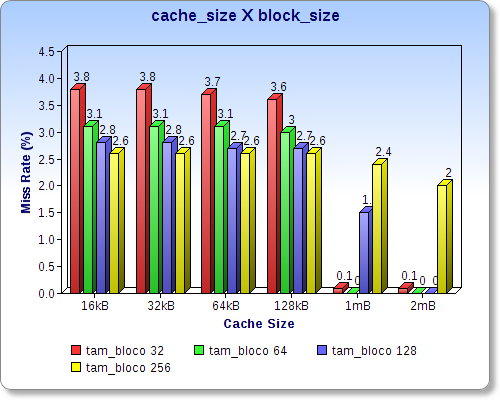
\includegraphics[width=100mm]{fig.png}
\caption{Resultados da Simulação}
\label{fig1}
\end{figure}

\subsection{Análise dos Resultados}

Observando os dados obtidos, podemos notar um acontecimento que parece estranho.
Com grande tamanho de bloco e de cache, a taxa de \emph{miss} aumenta. Depois
de muito quebrarmo a cabeça, concluímos que esse aumento na taxa de \emph{miss},
é devido ao fato de que com o tamanho de bloco maior, tu consegue referenciar
menos posições da memória, gerando mais \emph{miss} na hora de percorrer o grafo.

\section{Conclusão}

Para o problema abordado, os dois elementos que mais influenciam no desempenho
de memória são: O tamanho da cache e o aproveitamento dos dados acessados a cada
procura. Um tamanho de bloco maior não se provou melhor, já que para caches
grandes ele não demonstrou melhora de performance significativa.

\end{document}
